\documentclass[11pt,aspectratio=169]{beamer}
  % papersize={16cm,9cm},

\newcommand{\formula}{F}
\newcommand{\Obj}{\textsc{O}}
\newcommand{\inc}{\text{I}}
\newcommand{\dec}{\text{D}}
\newcommand{\var}{\textsc{var}}
\newcommand{\lit}{\textsc{lit}}
\newcommand{\Min}{\texttt{Minimize-\allowbreak{}Inc}}
\newcommand{\Simpr}{\texttt{Solution-\allowbreak{}Improving-\allowbreak{}Search}}
\newcommand{\E}{\texttt{EnumSols}}
\newcommand{\Ex}{\texttt{ExistsSol}}
\newcommand{\T}{\mathtt{T}}
\newcommand{\assumps}{\mathcal{A}}
\newcommand{\satsolver}{\texttt{isSAT}}
\newcommand{\res}{\text{res}}
\newcommand{\algname}{\textsc{BiOptSat}}
\newcommand{\tot}{\textsc{Tot}}
\newcommand{\ov}[2]{\langle #1 < #2 \rangle}
\newcommand{\ove}[2]{\langle #1 \leq #2 \rangle}
\newcommand{\satunsat}{\texttt{SAT-\allowbreak{}UNSAT}}
\newcommand{\unsatsat}{\texttt{UNSAT-\allowbreak{}SAT}}
\newcommand{\msu}{\texttt{MSU3}}
\newcommand{\I}{\mathcal{I}}
\newcommand{\Act}{\texttt{Act}}
\newcommand{\oll}{\texttt{OLL}}
\newcommand{\msh}{\texttt{MSHybrid}}
\newcommand{\hs}{\texttt{hs}}
\newcommand{\nsamp}{n}
\newcommand{\nfeat}{m}
\newcommand{\nclauses}{k}
\newcommand{\selector}{s}
\newcommand{\noise}{\eta}
\newcommand{\equals}{e}
\newcommand{\nelems}{n}
\newcommand{\nsets}{m}
\newcommand{\setcard}{s}
\newcommand{\elemprob}{p}
\newcommand{\sets}{\mathcal{S}}
\newcommand{\element}{e}
\newcommand{\cover}{\mathcal{C}}
\newcommand{\cost}{c}
\newcommand{\cores}{\mathcal{K}}
\newcommand{\core}{\kappa}
\newcommand{\sol}{\tau}
\newcommand{\scep}{SetCovering-EP}
\newcommand{\scsc}{SetCovering-SC}
\newcommand{\clause}{C}
\newcommand{\softs}{\textsc{S}}
\newcommand{\generalobj}{f}
\newcommand{\nobj}{p}
\newcommand{\feasible}{\mathcal{X}}
\newcommand{\decvar}{x}
\newcommand{\soloone}{\{i_2,\allowbreak d_1,\allowbreak d_3,\allowbreak d_4,\allowbreak \lnot i_1,\allowbreak \lnot i_3,\allowbreak \lnot i_4,\allowbreak \lnot d_2\}}
\newcommand{\solotwo}{\{i_1,\allowbreak i_2,\allowbreak d_1,\allowbreak d_2,\allowbreak \lnot i_3,\allowbreak \lnot i_4,\allowbreak \lnot d_3,\allowbreak \lnot d_4\}}
\newcommand{\solothree}{\{i_2,\allowbreak d_1,\allowbreak d_3,\allowbreak d_4,\allowbreak \lnot i_1,\allowbreak \lnot i_3,\allowbreak \lnot i_4,\allowbreak \lnot d_2\}}
\newcommand{\solcone}{\{i_1,\allowbreak i_2,\allowbreak i_3,\allowbreak i_4,\allowbreak d_1,\allowbreak d_2,\allowbreak d_3,\allowbreak d_4\}}
\newcommand{\solctwo}{\{i_1,\allowbreak i_2,\allowbreak d_1,\allowbreak d_2,\allowbreak d_3,\allowbreak d_4,\allowbreak \lnot i_3,\allowbreak \lnot i_4\}}
\newcommand{\solcthree}{\{i_2,\allowbreak d_1,\allowbreak d_2,\allowbreak d_3,\allowbreak d_4,\allowbreak \lnot i_1,\allowbreak \lnot i_3,\allowbreak \lnot i_4\}}
\newcommand{\solcfour}{\{i_1,\allowbreak i_2,\allowbreak i_3,\allowbreak d_1,\allowbreak d_2,\allowbreak \lnot i_4,\allowbreak \lnot d_3,\allowbreak \lnot d_4\}}
\newcommand{\solmcstrap}{\{i_1,\allowbreak i_3,\allowbreak i_4,\allowbreak d_1,\allowbreak d_3,\allowbreak d_4,\allowbreak \lnot i_2,\allowbreak \lnot d_2\}}
\newcommand{\TODO}[1]{\textcolor{red}{#1}}
\newcommand{\thr}{\texttt{thr}}
\newcommand{\NP}{$\mathcal{NP}$}

\mode<presentation>{}

%%%%%%%%%%%%%%%%%%%%%%%%%%%%%%
% Fill in the following information: AUTHOR, TITLE, DATE

\author{Christoph Jabs}
\title[\algname{}]{MaxSAT-Based Bi-Objective Boolean Optimization}
\date{10th April 2022}
\institute{HIIT, Department of Computer Science, University of Helsinki}

%%%%%%%%%%%%%%%%%%%%%%%%%%%%%%
% load packages
% add packages if needed

\usepackage[T1]{fontenc}
\usepackage[british]{babel}
\usepackage{amsmath,amsfonts,amssymb,amsthm}
\usepackage{color}
\usepackage[tracking=smallcaps, letterspace=-55]{microtype} % package for font spacing

\usepackage{transparent} % for setting opacity of pictures
\usepackage{pifont} % for checkmark (\ding{51}) and cross (\ding{55})
\usepackage{booktabs,array} % for tables
\usepackage{graphicx} % for figures
\graphicspath{{./img}} % to set the path of figures
\usepackage{algorithm}       % For pseudocode
\usepackage[noend]{algorithmic} % For pseudocode
\usepackage{appendixnumberbeamer}
\usepackage{cancel}

\usepackage{tikz}
\usetikzlibrary{overlay-beamer-styles}
\usetikzlibrary{patterns.meta}
\usetikzlibrary{calc}
\usepackage{pgfplots}
\pgfplotsset{compat=newest}
\usepgfplotslibrary{fillbetween}
\usepgfplotslibrary{groupplots}


%%%%%%%%%%%%%%%%%%%%%%%%%%%%%%
% set beamer colors

\definecolor{hyblue}{RGB}{0,155,255}
\setbeamercolor{alerted text}{fg=hyblue}
\setbeamercolor{structure}{fg=hyblue}
\setbeamercovered{transparent}

\setbeamertemplate{itemize item}{\color{hyblue}}

%%%%%%%%%%%%%%%%%%%%%%%%%%%%%%
% set font (helvetica plays the role of Arial)
\usepackage{helvet}
\renewcommand{\familydefault}{\sfdefault}

%%%%%%%%%%%%%%%%%%%%%%%%%%%%%%
% set frametitle

\setbeamercolor{frametitle}{fg=black}%{fg=hyblue}
\setbeamerfont{frametitle}{series=\bfseries, shape=\scshape, size=\huge}
\setbeamertemplate{frametitle}[default][left,leftskip=3.5cm] % left shift of frame title
\addtobeamertemplate{frametitle}{\vspace{0.5cm}}{\vspace{1cm}} % spacing above and below frame title

%%%%%%%%%%%%%%%%%%%%%%%%%%%%%%
% set footline and headline
\beamertemplatenavigationsymbolsempty
\setbeamertemplate{headline}{ }
\setbeamertemplate{footline}{%
	 \usebeamercolor[fg]{page number in head/foot}%
	 \usebeamerfont{page number in head/foot}%
	\hspace{0.5cm}	
	
\includegraphics[width=2.5cm]{HY__LC05_txt__L_3L_B3____BW_cropped}
	\hfill
	\insertshorttitle\ /\ \insertshortauthor	\hfill
	\insertshortdate	\hspace{0.5cm}
	\insertframenumber\,/\,\inserttotalframenumber \hspace{0.5cm} \vskip2pt%
}

%%%%%%%%%%%%%%%%%%%%%%%%%%%%%%
% Other style settings
\useinnertheme{circles}

%%%%%%%%%%%%%%%%%%%%%%%%%%%%%%
%%%%%%%%%%%%%%%%%%%%%%%%%%%%%%

% xfgs_normal6 colour palette
\definecolor{color0}{RGB}{64,83,211}
\definecolor{color1}{RGB}{221,179,16}
\definecolor{color2}{RGB}{181,29,20}
\definecolor{color3}{RGB}{0,190,255}
\definecolor{color4}{RGB}{251,73,176}
\definecolor{color5}{RGB}{0,178,93}
\definecolor{color6}{RGB}{202,202,202}

\newcommand<>{\xxcancel}[1]{\alt#2{\xcancel{#1}\vphantom{#1}}{#1}}

\begin{document}

{
\usebackgroundtemplate{
\setlength{\unitlength}{1cm}
\begin{picture}(16,9)
	\put(-0.1,5){ 
\includegraphics[width=4cm]{HY__LA01_Flame_____B3____BW} }
\end{picture}
\setlength{\unitlength}{1pt}
}
\setbeamertemplate{headline}{ }%
\begin{frame}[noframenumbering]{}
\vspace{1cm}
\hspace{3.5cm}
\begin{minipage}{10cm}
  {\huge \textcolor{hyblue}{\textbf{\inserttitle}}}
  \bigskip
\end{minipage}
\vspace{.5cm}
\begin{center}
{\large \insertauthor}
\bigskip

\emph{Supervisors}: Matti Järvisalo, Jeremias Berg, Andreas Niskanen \\
Constraint Reasoning and Optimization Research Group
\end{center}
\end{frame}
}

\usebackgroundtemplate{
\setlength{\unitlength}{1cm}
\begin{picture}(16,2.5)
\put(0.1,0){

\includegraphics[width=2.5cm]{HY__LA01_Flame_____B3____BW}\hfill
}
\end{picture}
\setlength{\unitlength}{1pt}
}

\section{Introduction}

\begin{frame}{Introduction}
  % Outline of the presentation
  % Paper under review for SAT 2022
  \begin{columns}
    \begin{column}{0.55\textwidth}
      {\LARGE
      MaxSAT-Based Bi-Objective Boolean Optimization
      }
      \medskip

      Paper under review at international scientific conference (SAT'22)
    \end{column}
    \begin{column}{0.35\textwidth}
      \begin{enumerate}
        \item Motivation
        \item Contribution (\algname{})
        \item Results
        \item Take away points
      \end{enumerate}
    \end{column}
  \end{columns}
\end{frame}

\section{Motivation}

\begin{frame}{Motivation --- Optimization}
  % Flat example single objective
  \begin{columns}
    \begin{column}{.48\textwidth}
      \emph{Task}: Choose the \alert<3|handout:0>{cheapest flat} with \alert<2|handout:0>{at least two rooms}

      \begin{block}<4->{What if...}
        ... we want to take commute into consideration as well?
      \end{block}
    \end{column}
    \begin{column}{.48\textwidth}
      \begin{center}
        \begin{tabular}{@{}crr@{}}
          \toprule
          Flat & Rooms & Price \\
          \midrule
          A & 2 & 300\,000 \texteuro \\
          \textbf<3->{B} & \textbf<3->{2} & \alert<3|handout:0>{\textbf<3->{240\,000 \texteuro}} \\
          \xxcancel<2->{C} & \alert<2|handout:0>{\xxcancel<2->{1}} & \xxcancel<2->{180\,000 \texteuro} \\
          D & 2 & 270\,000 \texteuro \\
          \bottomrule
        \end{tabular}
      \end{center}
    \end{column}
  \end{columns}
\end{frame}

\begin{frame}{Motivation --- Multiple Objectives}
  % Flat example multiple objectives
  \begin{columns}
    \begin{column}{.48\textwidth}
      \emph{Task}: Choose a flat with \alert<2|handout:0>{at least two rooms} that is as cheap as possible while also having \alert<1>{as short of a commute as possible}.

      \begin{block}<4->{Optimality for Multiple Objectives}
        There is no single definition of optimality for multiple objectives!
      \end{block}

      \begin{block}<5->{Pareto Optimality}
        All solutions for which no other solution is \alert{clearly} better are considered optimal
      \end{block}
    \end{column}
    \begin{column}{.48\textwidth}
      \begin{center}
        \begin{tabular}{@{}crrr@{}}
          \toprule
          Flat & Rooms & Price & Commute\\
          \midrule
          A & 2 & 300\,000 \texteuro & 4 km \\
          \textit<4->{\textbf<3|handout:0>{B}} & \textit<4->{\textbf<3|handout:0>{2}} & \textit<4->{\alert<3-4|handout:0>{\textbf<3|handout:0>{240\,000 \texteuro}}} & \textit<4->{\alert<3-4|handout:0>{\textbf<3|handout:0>{3 km}}} \\
          \xxcancel<2->{C} & \alert<2|handout:0>{\xxcancel<2->{1}} & \xxcancel<2->{180\,000 \texteuro} & \xxcancel<2->{3 km} \onslide<4->\\
          \textit<4->{D} & \textit<4->{2} & \textit<4->{\alert<4|handout:0>{270\,000 \texteuro}} & \textit<4->{\alert<4|handout:0>{2 km}} \\
          \bottomrule
        \end{tabular}
      \end{center}
    \end{column}
  \end{columns}
\end{frame}

\begin{frame}{Motivation --- Implicit Solution Set}
  % Decision tree example
  \begin{columns}
    \begin{column}{.48\textwidth}
      \emph{Task}: From all valid decision trees, find the smallest ones that also minimize classification error

      \begin{block}<4->{Hard Problems}
        Implicit solution definitions are $\mathcal{NP}$-hard for many real-world problems
      \end{block}
    \end{column}
    \begin{column}{.15\textwidth}
      \begin{center}
        \begin{tabular}{@{}cc@{\hspace{1.5em}}c@{}}
          \toprule
          $x_1$ & $x_2$ & $y$ \\
          \midrule
          1 & 1 & 1 \\
          0 & 1 & 0 \\
          1 & 0 & 0 \\
          \bottomrule
        \end{tabular}
      \end{center}
    \end{column}
    \begin{column}{.25\textwidth}
      \begin{center}
        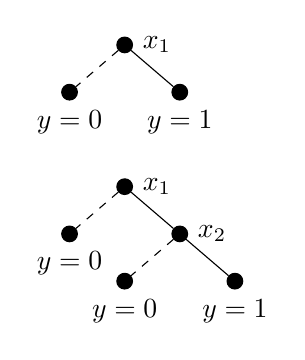
\begin{tikzpicture}
          \onslide<2->{
            \node (1n1) [circle,draw,fill,inner sep=2pt,label=right:$x_1$] at (0,0) {};
            \node (1n2) [circle,draw,fill,inner sep=2pt,label={below:$y=0$}] at (-0.7,-0.6) {};
            \node (1n3) [circle,draw,fill,inner sep=2pt,label={below:$y=1$}] at (0.7,-0.6) {};
            \draw [dashed] (1n1) -- (1n2);
            \draw (1n1) -- (1n3);
          }

          \onslide<3->{
            \node (1n1) [circle,draw,fill,inner sep=2pt,label=right:$x_1$] at (0,-1.8) {};
            \node (1n2) [circle,draw,fill,inner sep=2pt,label={below:$y=0$}] at (-0.7,-2.4) {};
            \node (1n3) [circle,draw,fill,inner sep=2pt,label={right:$x_2$}] at (0.7,-2.4) {};
            \node (1n4) [circle,draw,fill,inner sep=2pt,label={below:$y=0$}] at (0,-3.0) {};
            \node (1n5) [circle,draw,fill,inner sep=2pt,label={below:$y=1$}] at (1.4,-3.0) {};
            \draw [dashed] (1n1) -- (1n2);
            \draw (1n1) -- (1n3);
            \draw [dashed] (1n3) -- (1n4);
            \draw (1n3) -- (1n5);
          }
        \end{tikzpicture}
      \end{center}
    \end{column}
  \end{columns}
\end{frame}

\section{Contribution}

\begin{frame}{Thesis Contribution}
  % Development of BiOptSat
  % Evaluation of 5 variants and comparison to two existing approaches
  \begin{itemize}
    \item Development of the \alert<2>{\algname{} algorithm}
    \begin{itemize}
      \item Enumeration of exact \alert<2>{Pareto-optimal} solutions to \alert<2>{hard problems}
    \end{itemize}
    \item \alert<3>{Implementation} of the \algname{} algorithm and its competitors \\ {\small (will be released open source)}
    \item \alert<4>{Evaluation of variants} of \algname{} and comparison to two competitors
    \item \alert<5>{Evaluation of refinements} to \algname{}
  \end{itemize}
\end{frame}

\begin{frame}{High-Level Overview of \algname{}}
  % Declarative approach to solving problems
  % Search progress of lexicographic method
  \begin{columns}
    \begin{column}{.65\textwidth}
      \begin{centering}
        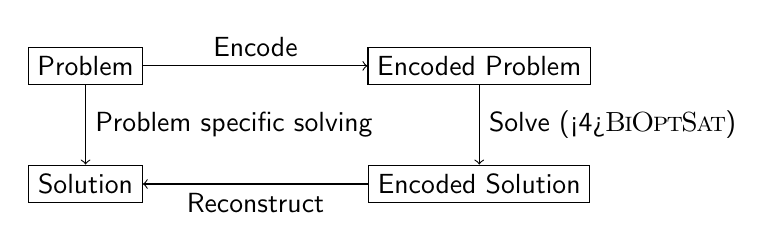
\begin{tikzpicture}
          \node (p) [draw] at (0,0) {Problem};
          \onslide<3->{
            \node (fp) [draw] at (5,0) {Encoded Problem};
            \node (fs) [draw] at (5,-1.5) {Encoded Solution};
          }
          \node (s) [draw] at (0,-1.5) {Solution};

          \onslide<3->{
            \draw [->] (p) -- (fp) node [midway,above] {Encode};
            \draw [->] (fp) -- (fs) node [midway,right] {Solve (\alert<4>{\algname{}})};
            \draw [->] (fs) -- (s) node [midway,below] {Reconstruct};
          }
          \onslide<2|handout:0>{
            \draw [->] (p) -- (s) node [midway,right] {Problem specific solving};
          }
        \end{tikzpicture}
      \end{centering}
    \end{column}
    \begin{column}{.31\textwidth}
      \onslide<4->{
        \begin{itemize}
          \item Encoding language: Boolean logic
          \item Lexicographic method
          \item Based on MaxSAT algorithms
          \item Making use of so-called SAT solver
        \end{itemize}
      }
    \end{column}
  \end{columns}
\end{frame}

\begin{frame}{Search Progression of \algname{}}
  % Step by step search trace
  \begin{columns}
    \begin{column}{.48\textwidth}
      \begin{center}
        \begin{tikzpicture}
          \def\axmax{4.5}
            \begin{axis}[
              width=5.5cm,
              height=5.5cm,
              label style={font=\small},
              tick label style={font=\small},
              legend style={
                anchor=north west,
                at={(1.05,0.9)},
                font=\footnotesize,
                fill opacity=0.8,
                draw opacity=1,
                text opacity=1
              },
              tick pos=left,
              xlabel={$\textsc{O}_\text{I}$},
              ylabel={$\textsc{O}_\text{D}$},
              xmin=0,
              xmax=4,
              ymin=0,
              ymax=4,
              axis x line*=bottom,
              axis y line*=left,
              xtick={0,1,2,3,4},
              ytick={0,1,2,3,4},
            ]

            \addplot [color6,name path=border,forget plot] coordinates {(1,4) (1,2) (2,2) (2,1) (4,1)};
            \path [name path=axis] (1,4) -- (0,4) -- (0,0) -- (4,0) -- (4,1);
            \addplot [color6,pattern={Lines[angle=-45, line width=.3pt]}, pattern color=color6] fill between [of=border and axis];


            \only<2->{
              \node [label=$\tau^c_1$] at (3,3) {};
              \addplot [only marks,color3, mark=o] coordinates {(3,3)};
            }

            \only<3|handout:0>{
              \addplot [color5,name path=dom] coordinates {(3,1) (3,3) (1,3)};
              \addplot [color5,pattern={Lines[angle=45, line width=.3pt]}, pattern color=color5] fill between [of=dom and border];

              \addplot [only marks,color3, mark=*] coordinates {(1,2) (2,1)};

              \node [label=left:$\tau^o_1$] at (1,2) {};
              \node [label=below:$\tau^o_2$] at (2,1) {};
            }

            \only<4->{
              \node [label=$\tau^c_2$] at (2,3) {};
              \addplot [only marks,color3, mark=o] coordinates {(2,3)};
              \draw [semithick,dashed, color0, ->, shorten >=3pt, shorten <=3pt] (3,3) to[out=155, in=25] (2,3);
            }

            \only<5->{
              \node [label=left:$\tau^c_3$] at (1,3) {};
              \addplot [only marks,color3, mark=o] coordinates {(1,3)};
              \draw [semithick,dashed, color0, ->, shorten >=3pt, shorten <=3pt] (2,3) to[out=155, in=25] (1,3);
            }

            \only<6->{
              \node [label=left:$\tau^o_1$] at (1,2) {};
              \addplot [only marks,color3, mark=*] coordinates {(1,2)};
              \draw [semithick,dashdotted, color1, ->, shorten >=3pt, shorten <=3pt] (1,3) to[out=-75, in=75] (1,2);
            }

            \only<7->{
              \node [label=below:$\tau^c_4$] at (3,1) {};
              \addplot [only marks,color3, mark=o] coordinates {(3,1)};
              \draw [semithick,dashdotdotted, color5, ->, shorten >=3pt, shorten <=3pt] (1,2) to[out=25, in=110] (3,1);
            }

            \only<8->{
              \node [label=below:$\tau^o_2$] at (2,1) {};
              \addplot [only marks,color3, mark=*] coordinates {(2,1)};
              \draw [semithick,dashed, color0, ->, shorten >=3pt, shorten <=3pt] (3,1) to[out=155, in=25] (2,1);
            }
          \end{axis}
        \end{tikzpicture}
      \end{center}
    \end{column}
    \begin{column}{.48\textwidth}
      \onslide<9->{
        \begin{itemize}
          \item Ordered enumeration from top left to bottom right
        \end{itemize}
      }
    \end{column}
  \end{columns}
\end{frame}

\section{Results}

\begin{frame}{Results --- Solved Instances}
  % Cactus
  Benchmark: Learning Pareto-optimal decision rules
  \begin{center}
    \begin{tikzpicture}
      \def\xcut{210}
      \begin{groupplot}[
        group style={
          group size=2 by 1,
          xlabels at=edge bottom,
          ylabels at=edge left,
        },
        label style={font=\small},
        tick label style={font=\small},
        scaled y ticks={base 10:-3},
        legend style={
          anchor=north east,
          at={(3.2,1)},
          font=\footnotesize,
          fill opacity=0.8,
          draw opacity=1,
          text opacity=1
        },
        tick pos=left,
        xlabel={\# instances solved},
        ylabel={cpu time (s)},
        height=5cm,
        width=5cm,
        ytick={0,1000,2000,3000,4000,5000},
        yticklabels={0,1,2,3,4,},
        extra y ticks={5400},
        extra y tick labels={5.4},
      ]
        \nextgroupplot[
          xmin=70,
          xmax=223,
          ymin=0,
          ymax=5400,
          axis x line*=bottom,
          axis y line*=left,
          xtick={100,150,200},
          xticklabels={100,150,},
          extra x ticks={70,223},
        ]

        \coordinate (orig window start) at ({rel axis cs: 1,1}-|{axis cs:\xcut,0});
        \coordinate (orig window end) at (rel axis cs: 1,1);

        \only<4->{
          \addplot [semithick,color0,solid,mark=asterisk,forget plot] table [x=nsolved,y=bioptsat-msh,col sep=comma] {../plots/mlic-cactus-single.csv};
        }
        \addlegendimage{color0,solid,semithick,mark=asterisk}
        \addlegendentry{\algname}

        \only<3->{
          \addplot [semithick,color5,dashed,mark=x,forget plot] table [x=nsolved,y=pminimal,col sep=comma] {../plots/mlic-cactus-single.csv};
        }
        \addlegendimage{color5,dashed,semithick,mark=x}
        \addlegendentry{Competitor 1}

        \only<2->{
          \addplot [semithick,color6,dashdotted,mark=o,forget plot] table [x=nsolved,y=seesaw,col sep=comma] {../plots/mlic-cactus-single.csv};
        }
        \addlegendimage{color6,dashdotted,semithick,mark=o}
        \addlegendentry{Competitor 2}

        \nextgroupplot[
          xmin=\xcut,
          xmax=223,
          ymin=0,
          ymax=5400,
          axis x line*=bottom,
          axis y line*=left,
          xtick={\xcut,215,220},
          extra x ticks={223},
        ]

        \coordinate (zoom window start) at (rel axis cs: 0,1);
        \coordinate (zoom window end) at (rel axis cs: 1,1);

        \only<4->{
          \addplot [semithick,color0,solid,mark=asterisk] table [x=nsolved,y=bioptsat-msh,col sep=comma] {../plots/mlic-cactus-single.csv};
        }

        \only<3->{
          \addplot [semithick,color5,solid,mark=x] table [x=nsolved,y=pminimal,col sep=comma] {../plots/mlic-cactus-single.csv};
        }
      \end{groupplot}

      \draw ($(orig window start) +(0,12pt)$) -- ++(0,3pt) -- ($(orig window end) +(0,15pt)$) -- ++(0,-3pt);
      \draw ($($(orig window start) +(0,15pt)$)!.5!($(orig window end) +(0,15pt)$)$) -- ++(0,3pt) -- ($($($(zoom window start) +(0,15pt)$)!.5!($(zoom window end) +(0,15pt)$)$) +(0,3pt)$) -- ++(0,-3pt);
      \draw ($(zoom window start) +(0,12pt)$) -- ++(0,3pt) -- ($(zoom window end) +(0,15pt)$) -- ++(0,-3pt);
    \end{tikzpicture}
  \end{center}
\end{frame}

\begin{frame}{Results --- Instance Runtimes}
  % MSH scatter
  \begin{columns}
    \begin{column}{.48\textwidth}
      \begin{centering}
        \begin{tikzpicture}
          \begin{loglogaxis}[
            width=5.5cm,
            height=5.5cm,
            label style={font=\small},
            tick label style={
              font=\small,
              /pgf/number format/1000 sep=\,,
            },
            legend style={
              legend pos=north west,
              font=\footnotesize,
              fill opacity=0.8,
              draw opacity=1,
              text opacity=1
            },
            tick pos=left,
            xlabel={Competitor 1 (s)},
            ylabel={\algname{} (s)},
            xmin=30,
            xmax=5400,
            ymin=30,
            ymax=5400,
            log ticks with fixed point,
            axis x line*=bottom,
            axis y line*=left,
            xtickten={2,3},
            ytickten={2,3},
            extra x ticks={30,5400},
            extra y ticks={30,5400},
            extra x tick labels={30,5\,400},
            extra y tick labels={30,5\,400},
            minor xtick={70,80,90,200,300,400,500,600,700,800,900,2000,3000,4000},
            minor ytick={40,50,60,70,80,90,200,300,400,500,600,700,800,900,2000,3000,4000},
          ]

          \draw [dotted] (30,30) -- (5400,5400);
          \draw [loosely dotted] (60,30) -- (5400,2700);
          \draw [loosely dotted] (30,60) -- (2700,5400);

          \only<3->{
            \addplot [only marks,color0,mark=x,forget plot] table [x=pminimal,y=bioptsat-msh,col sep=comma] {../plots/setcover-element-prob-msh-scatter-single.csv};
          }
          \addlegendimage{only marks,color0,mark=x}
          \addlegendentry{SetCovering 1}

          \only<4->{
            \addplot [only marks,color1,mark=o,forget plot] table [x=pminimal,y=bioptsat-msh,col sep=comma] {../plots/setcover-set-card-msh-scatter-single.csv};
          }
          \addlegendimage{only marks,color1,mark=o}
          \addlegendentry{SetCovering 2}

          \only<2->{
            \addplot [only marks,color2,mark=+,forget plot] table [x=pminimal,y=bioptsat-msh,col sep=comma] {../plots/mlic-msh-scatter-single.csv};
          }
          \addlegendimage{only marks,color2,mark=+}
          \addlegendentry{Decision Rules}

          \end{loglogaxis}
        \end{tikzpicture}
      \end{centering}
    \end{column}
    \begin{column}{.48\textwidth}
      \onslide<5->{
        \begin{itemize}
          \item \algname{} outperformed both competitors
          \item Amount of outperforming competitors depends on benchmark
        \end{itemize}
      }
    \end{column}
  \end{columns}
\end{frame}

\section{Take Away Points}

\begin{frame}{Take Away Points}
  % Start with a summer internship!
  \begin{columns}
    \begin{column}{.48\textwidth}
      \begin{block}{Content of Thesis}
        \begin{itemize}
          \item Paper in review: significant result for a thesis project
          \item (Exact) bi-objective optimization is interesting and not that well researched
        \end{itemize}
      \end{block}
    \end{column}
    \begin{column}{.48\textwidth}
      \begin{block}{Thesis Process}
        \begin{itemize}
          \item Starting with a summer internship is great
          \item Working as a research assistant allows for diving deep into a topic
        \end{itemize}
      \end{block}
    \end{column}
  \end{columns}
\end{frame}

{
\usebackgroundtemplate{
\transparent{0.3} % requires \usepackage{transparent} & compile twice
\setlength{\unitlength}{1cm}
\begin{picture}(16,9)
\put(0.2,1){
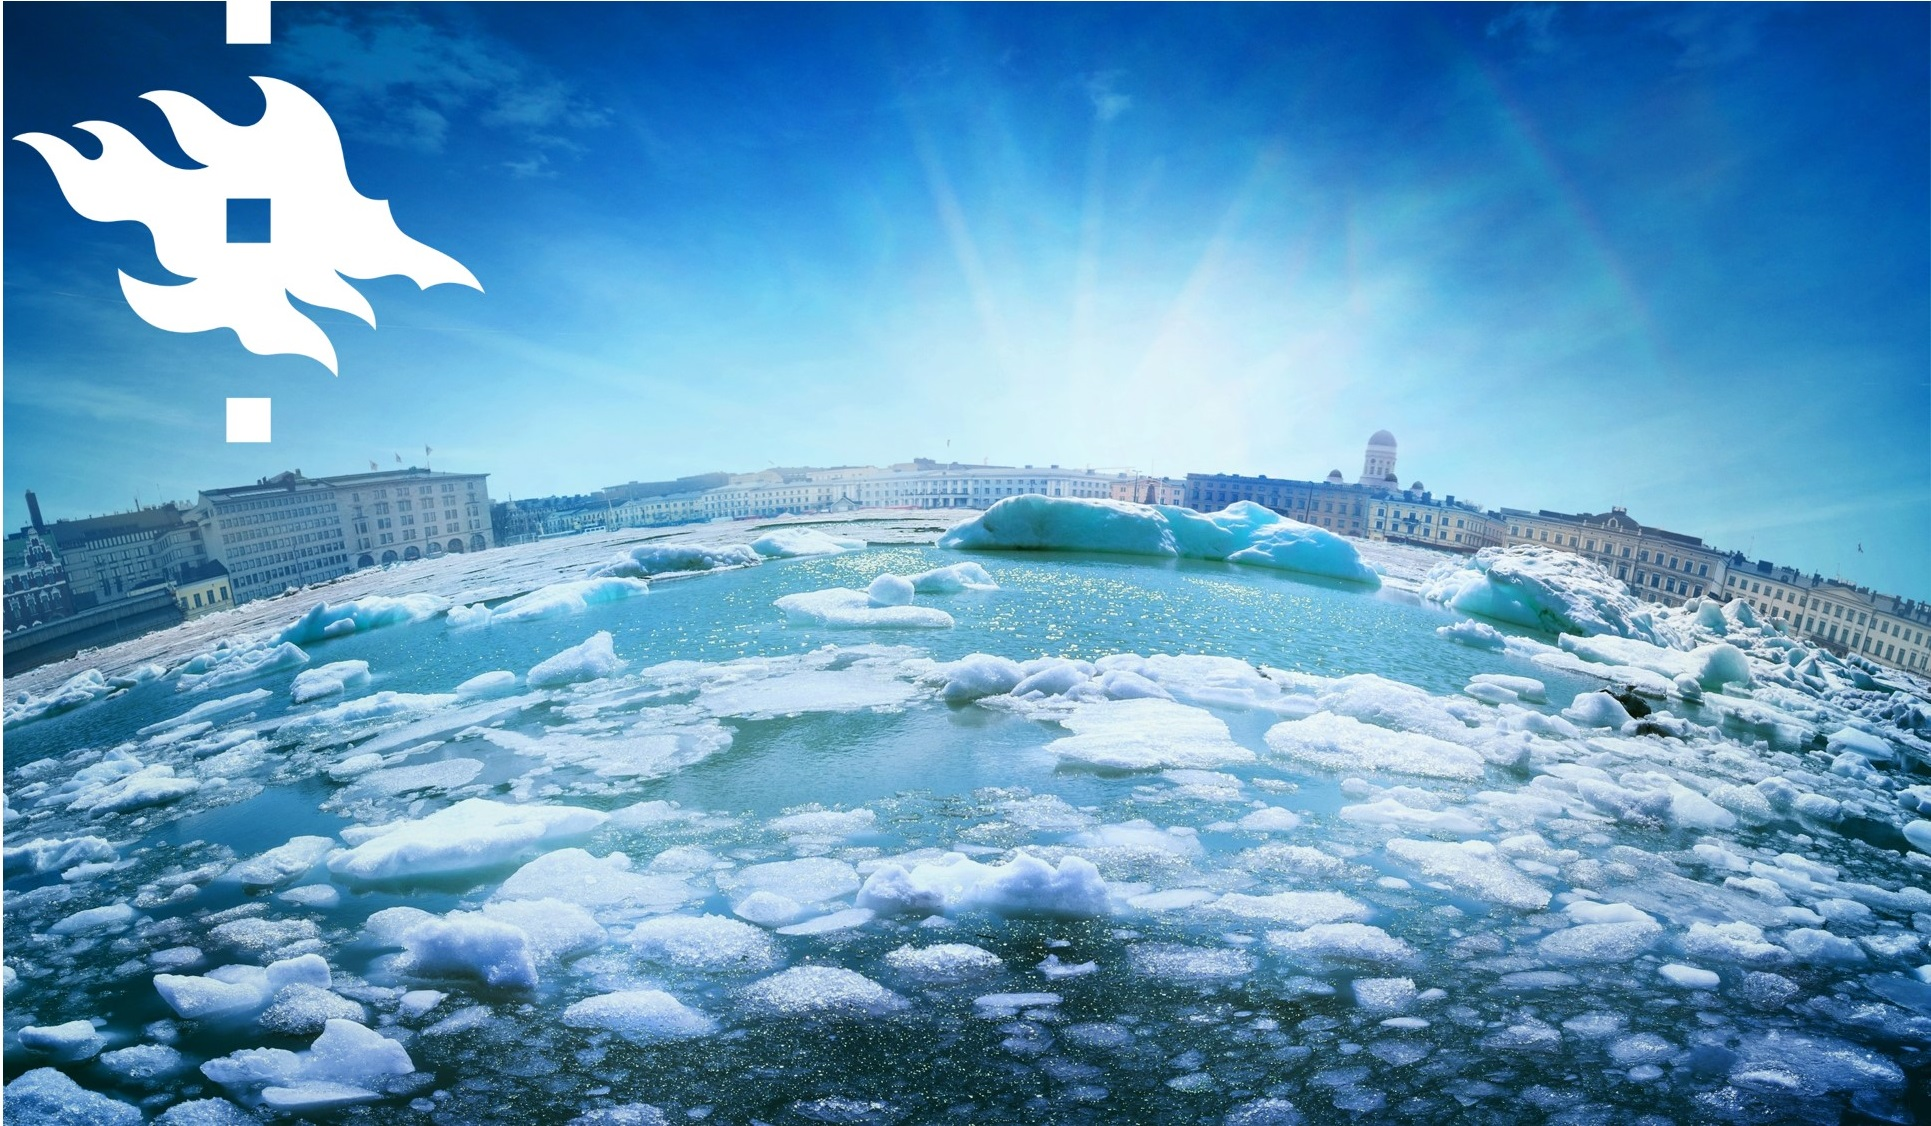
\includegraphics[width=15cm,height=7.5cm]{hy_brand_image_1_wide_background_hires_logo}
}
\end{picture}
\setlength{\unitlength}{1pt}
}

\begin{frame}
  \centering
  \LARGE
  Thank you for your attention!
\end{frame}
}

\appendix

\begin{frame}{Pareto Optimality}
  \begin{definition}[Domination]
    Given two objective functions $\Obj_1,\Obj_2$ and two solutions $\sol,\sol'$, $x$ dominates $\sol'$ if (i)~$\Obj_i(\sol) \leq \Obj_i(\sol')$ for all $i\in\{1,2\}$, and (ii)~$\Obj_i(\sol) < \Obj_i(\sol')$ for some $i\in\{1,2\}$.
    We represent $\sol$ dominating $\sol'$ as $\sol \prec \sol'$.
  \end{definition}

  \begin{definition}[Pareto optimality]
    A solution $\sol$ is Pareto-optimal iff there is no $\sol'$ such that $\sol' \prec \sol$, i.e., $\sol$ is not dominated by any other solution.
  \end{definition}
\end{frame}

\begin{frame}{\algname{}}
  \begin{algorithm}[H]
    \caption{\algname{}: MaxSAT-based bi-objective optimization}
    \textbf{Input}: A formula $\formula$, two objectives $\Obj_\inc$ and $\Obj_\dec$.\\
    \textbf{Output}: Either one or all Pareto-optimal solution for each Pareto point of $\formula$.

    \begin{algorithmic}[1]
      \STATE $\sol^r \gets \texttt{InitSATsolverAndSolve}(F)$ \quad\COMMENT{Invokes the SAT solver on the formula.}
      \STATE $b_\dec \gets \infty, b_\inc \gets 0$
      \WHILE{$\res = \text{SAT}$}
      \STATE $(b_\inc, \sol^r) \gets \Min(b_\dec , \Obj_\inc(\sol^r))$  \quad\COMMENT{Maintains $\tot(\Obj_\inc)$ (or similar)}
      \STATE $(b_\dec, \sol^r) \gets  \Simpr(b_\inc , \Obj_\dec(\sol^r))$  \quad\COMMENT{Builds $\tot(\Obj_\dec)$}
      \STATE \textbf{yield} $\sol^r$  \quad\COMMENT{Optionally:  \textbf{yield} $\E(b_\dec, b_\inc)$}
      \STATE $(\res, \sol^r) \gets \satsolver(\{\ov{\Obj_\dec}{b_\dec}\})$
      \ENDWHILE
    \end{algorithmic}
  \end{algorithm}
\end{frame}

\begin{frame}{Search Details of \algname{}}
  % Step by step search trace
  \begin{columns}
    \begin{column}{.48\textwidth}
      \begin{center}
        \begin{tikzpicture}
          \def\axmax{4.5}
            \begin{axis}[
              width=5.5cm,
              height=5.5cm,
              label style={font=\small},
              tick label style={font=\small},
              legend style={
                anchor=north west,
                at={(1.05,0.9)},
                font=\footnotesize,
                fill opacity=0.8,
                draw opacity=1,
                text opacity=1
              },
              tick pos=left,
              xlabel={$\textsc{O}_\text{I}$},
              ylabel={$\textsc{O}_\text{D}$},
              xmin=0,
              xmax=4,
              ymin=0,
              ymax=4,
              axis x line*=bottom,
              axis y line*=left,
              xtick={0,1,2,3,4},
              ytick={0,1,2,3,4},
            ]

            \addplot [color6,name path=border,forget plot] coordinates {(1,4) (1,2) (2,2) (2,1) (4,1)};
            \path [name path=axis] (1,4) -- (0,4) -- (0,0) -- (4,0) -- (4,1);
            \addplot [color6,pattern={Lines[angle=-45, line width=.3pt]}, pattern color=color6] fill between [of=border and axis];


            \only<2-4|handout:0>{
              \node [label=$\tau^c_1$] at (3,3) {};
              \addplot [only marks,color3, mark=o] coordinates {(3,3)};
            }

            \only<3|handout:0>{
              \addplot [color5,name path=dom] coordinates {(3,1) (3,3) (1,3)};
              \addplot [color5,pattern={Lines[angle=45, line width=.3pt]}, pattern color=color5] fill between [of=dom and border];

              \addplot [only marks,color3, mark=*] coordinates {(1,2) (2,1)};

              \node [label=left:$\tau^o_1$] at (1,2) {};
              \node [label=below:$\tau^o_2$] at (2,1) {};
            }

            \only<4-5|handout:0>{
              \addplot [color2,name path=block] coordinates {(2.8,0) (2.8,4)};
              \path [name path=right] (2.8,0) -- (4,0) -- (4,4) -- (2.8,4);
              \addplot [color2,pattern={Lines[angle=45, line width=.3pt]}, pattern color=color2] fill between [of=block and right];
            }

            \only<5-7|handout:0>{
              \node [label=$\tau^c_2$] at (2,3) {};
              \addplot [only marks,color3, mark=o] coordinates {(2,3)};
            }

            \only<6-7|handout:0>{
              \addplot [color2,name path=block] coordinates {(1.8,0) (1.8,4)};
              \path [name path=right] (1.8,0) -- (4,0) -- (4,4) -- (1.8,4);
              \addplot [color2,pattern={Lines[angle=45, line width=.3pt]}, pattern color=color2] fill between [of=block and right];
            }

            \only<7-9|handout:0>{
              \node [label=left:$\tau^c_3$] at (1,3) {};
              \addplot [only marks,color3, mark=o] coordinates {(1,3)};
            }

            \only<8-9|handout:0>{
              \addplot [color2,name path=block] coordinates {(1.8,0) (1.8,2.8) (0,2.8)};
              \path [name path=topright] (1.8,0) -- (4,0) -- (4,4) -- (0,4) -- (0,2.8);
              \addplot [color2,pattern={Lines[angle=45, line width=.3pt]}, pattern color=color2] fill between [of=block and topright];
            }

            \only<9-11|handout:0>{
              \node [label=left:$\tau^o_1$] at (1,2) {};
              \addplot [only marks,color3, mark=*] coordinates {(1,2)};
            }

            \only<10-11|handout:0>{
              \addplot [color2,name path=block] coordinates {(4,1.8) (0,1.8)};
              \path [name path=top] (4,1.8) -- (4,4) -- (0,4) -- (0,1.8);
              \addplot [color2,pattern={Lines[angle=45, line width=.3pt]}, pattern color=color2] fill between [of=block and top];
            }

            \only<11-13|handout:0>{
              \node [label=below:$\tau^c_4$] at (3,1) {};
              \addplot [only marks,color3, mark=o] coordinates {(3,1)};
            }

            \only<12-13|handout:0>{
              \addplot [color2,name path=block] coordinates {(2.8,0) (2.8,1.8) (0,1.8)};
              \path [name path=topright] (2.8,0) -- (4,0) -- (4,4) -- (0,4) -- (0,1.8);
              \addplot [color2,pattern={Lines[angle=45, line width=.3pt]}, pattern color=color2] fill between [of=block and topright];
            }

            \only<13|handout:0>{
              \node [label=below:$\tau^o_2$] at (2,1) {};
              \addplot [only marks,color3, mark=*] coordinates {(2,1)};
            }

            \only<14->{
              \addplot [only marks,color3, mark=o] coordinates {(3,3) (2,3) (1,3) (3,1)};
              \addplot [only marks,color3, mark=*] coordinates {(1,2) (2,1)};

              \draw [semithick,dashed, color0, ->, shorten >=3pt, shorten <=3pt] (3,3) to[out=155, in=25] (2,3);
              \draw [semithick,dashed, color0, ->, shorten >=3pt, shorten <=3pt] (2,3) to[out=155, in=25] (1,3);
              \draw [semithick,dashdotted, color1, ->, shorten >=3pt, shorten <=3pt] (1,3) to[out=-75, in=75] (1,2);
              \draw [semithick,dashdotdotted, color5, ->, shorten >=3pt, shorten <=3pt] (1,2) to[out=25, in=110] (3,1);
              \draw [semithick,dashed, color0, ->, shorten >=3pt, shorten <=3pt] (3,1) to[out=155, in=25] (2,1);

              \node [label=$\tau^c_1$] at (3,3) {};
              \node [label=$\tau^c_2$] at (2,3) {};
              \node [label=left:$\tau^c_3$] at (1,3) {};
              \node [label=left:$\tau^o_1$] at (1,2) {};
              \node [label=below:$\tau^c_4$] at (3,1) {};
              \node [label=below:$\tau^o_2$] at (2,1) {};
            }
          \end{axis}
        \end{tikzpicture}
      \end{center}
    \end{column}
    \begin{column}{.48\textwidth}
      \onslide<13->{
        \begin{itemize}
          \item Progression from top left to bottom right
        \end{itemize}
      }
    \end{column}
  \end{columns}
\end{frame}

\end{document}
